\newcommand{\Harmonization}{
  \begin{figure}
    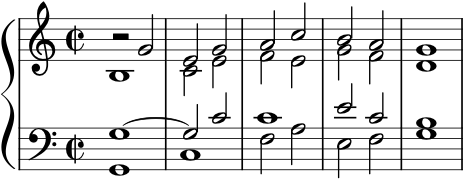
\includegraphics[width=5.5cm]{fig/piston.png}
    \hspace{1cm}
    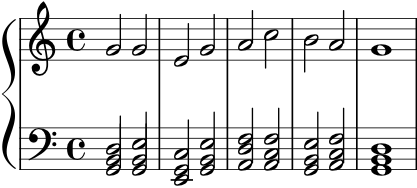
\includegraphics[width=5cm]{fig/fharm.png}
    \caption{Harmonization by Piston (left) and \fharm (right)}
    \Description{Harmonization by Piston (left) and \fharm (right)}
    \label{fig:harmonization}
  \end{figure}
}

\section{Harmony}
\label{sec:harmony}

TODO: Harmonize melody, use counterpoint for voice leading and to contrain harmony.
Mention grid for harmonic analsis, makes use of vectors.

\Harmonization
